\setcounter{section}{24}
\setcounter{subsection}{4}
\setcounter{subsubsection}{2}

% Copyright 2018 by Till Tantau
%
% This file may be distributed and/or modified
%
% 1. under the LaTeX Project Public License and/or
% 2. under the GNU Free Documentation License.
%
% See the file doc/generic/pgf/licenses/LICENSE for more details.


\section{Transformations\\变换}

\pgfname\ has a powerful transformation mechanism that is similar to the
transformation capabilities of \textsc{metafont}. The present section explains
how you can access it in \tikzname.

\pgfname\ 具有强大的变换机制,类似于 \textsc{metafont} 的变换能力。本节将解释您如何在 \tikzname\ 中访问它。


\subsection{The Different Coordinate Systems\\不同的坐标系}

It is a long process from  a coordinate like, say, $(1,2)$ or
$(1\mathrm{cm},5\mathrm{pt})$, to the position a point is finally placed on the
display or paper. In order to find out where the point should go, it is
constantly ``transformed'', which means that it is mostly shifted around and
possibly rotated, slanted, scaled, and otherwise mutilated.

从像 $(1,2)$ 或 $(1\mathrm{cm},5\mathrm{pt})$ 这样的坐标到最终放置在显示器或纸张上的位置是一个漫长的过程。为了找出点应该放在哪里,它不断地“变换”,这意味着它大多是被平移和可能被旋转、倾斜、缩放和其他方式改变。In detail, (at least) the following transformations are applied to a coordinate

like $(1,2)$ before a point on the screen is chosen:

具体来说,至少在选择屏幕上的点之前,会对像 $(1,2)$ 这样的坐标应用以下变换:%
\begin{enumerate}
    \item \pgfname\ interprets a coordinate like $(1,2)$  in its
        $xy$-coordinate system as ``add the current $x$-vector once and the
        current $y$-vector twice to obtain the new point''.

        \pgfname\ 在其 $xy$ 坐标系中将像 $(1,2)$ 这样的坐标解释为“将当前的 $x$ 向量加一次和当前的 $y$ 向量加两次以得到新的点”。

        \item \pgfname\ applies its coordinate transformation matrix to the
        resulting coordinate. This yields the final position of the point
        inside the picture.

        \pgfname\ 将其坐标变换矩阵应用于得到的坐标。这将给出图片中点的最终位置。

        \item The backend driver (like |dvips| or |pdftex|) adds transformation
        commands such that the coordinate is shifted to the correct position in
        \TeX's page coordinate system.

后端驱动程序(如 |dvips| 或 |pdftex|)添加变换命令,以便在 \TeX 的页面坐标系中将坐标移动到正确的位置。

    \item \textsc{pdf} (or PostScript) apply the canvas transformation matrix
        to the point, which can once more change the position on the page.

        \textsc{pdf}(或 PostScript)将画布变换矩阵应用于该点,这可能再次改变页面上的位置。

        \item The viewer application or the printer applies the device
        transformation matrix to transform the coordinate to its final pixel
        coordinate on the screen or paper.

        查看应用程序或打印机将设备变换矩阵应用于该坐标,将其变换为屏幕或纸张上的最终像素坐标。


    \end{enumerate}

In reality, the process is even more involved, but the above should give the
idea: A point is constantly transformed by changes of the coordinate system.

实际上,这个过程更加复杂,但上述内容应该给出了一个概念:点不断地通过坐标系统的变化进行变换。

In \tikzname, you only have access to the first two coordinate systems: The
$xy$-coordinate system and the coordinate transformation matrix (these will be
explained later). \pgfname\ also allows you to change the canvas transformation
matrix, but you have to use commands of the core layer directly to do so and
you ``better know what you are doing'' when you do this. The moment you start
modifying the canvas matrix, \pgfname\ immediately loses track of all
coordinates and shapes, anchors, and bounding box computations will no longer
work.

在 \tikzname\ 中,您只能访问前两个坐标系:$xy$ 坐标系和坐标变换矩阵(稍后将对此进行解释)。\pgfname\ 还允许您更改画布变换矩阵,但您必须直接使用核心层的命令来执行此操作,并且当您执行此操作时,“最好知道自己在做什么”。一旦开始修改画布矩阵,\pgfname\ 立即无法追踪所有坐标和形状,锚点和边界框计算将不再起作用。


\subsection{The XY- and XYZ-Coordinate Systems\\XY-和XYZ-坐标系}
\label{section-xyz}

The first and easiest coordinate systems are \pgfname's $xy$- and
$xyz$-coordinate systems. The idea is very simple: Whenever you specify a
coordinate like |(2,3)| this means $2v_x + 3v_y$, where $v_x$ is the current
\emph{$x$-vector} and $v_y$ is the current \emph{$y$-vector}. Similarly, the
coordinate |(1,2,3)| means $v_x + 2v_y + 3v_z$.

最简单的坐标系是\pgfname 的 $xy$-和 $xyz$-坐标系。其思想非常简单:每当您指定像 |(2,3)| 这样的坐标时,它的意思是 $v_x + 3v_y$,其中 $v_x$ 是当前的\emph{$x$-向量},$v_y$ 是当前的\emph{$y$-向量}。类似地,坐标 |(1,2,3)| 的意思是 $v_x + 2v_y + 3v_z$。

Unlike other packages, \pgfname\ does not insist that $v_x$ actually has a
$y$-component of $0$, that is, that it is a horizontal vector. Instead, the
$x$-vector can point anywhere you want. Naturally, \emph{normally} you will
want the $x$-vector to point horizontally.

与其他包不同,\pgfname 不坚持 $v_x$ 实际上有一个 $y$-分量为 $0$,也就是说,它是一个水平向量。相反,$x$-向量可以指向您想要的任何位置。当然,\emph{通常}情况下,您希望 $x$-向量指向水平方向。

One undesirable effect of this flexibility is that it is not possible to
provide mixed coordinates as in $(1,2\mathrm{pt})$. Life is hard.

这种灵活性的一个不良影响是无法提供混合的坐标,比如 $(1,2\mathrm{pt})$。生活是艰难的。

To change the $x$-, $y$-, and $z$-vectors, you can use the following options:

要更改 $x$、$y$ 和 $z$-向量,可以使用以下选项:

\begin{key}{/tikz/x=\meta{value} (initially 1cm)}
    If \meta{value} is a dimension, the $x$-vector of \pgfname's
    $xyz$-coordinate system is set up to point \meta{value} to the right, that
    is, to $(\meta{value},0pt)$.
    %

    如果 \meta{value} 是一个尺寸,\pgfname 的 $xyz$-坐标系的 $x$-向量将设置为向右指向 \meta{value},也就是 $(\meta{value},0\mathrm{pt})$。

    \begin{codeexample}[]
\begin{tikzpicture}
  \draw                  (0,0)   -- +(1,0);
  \draw[x=2cm,color=red] (0,0.1) -- +(1,0);
\end{tikzpicture}
\end{codeexample}

\begin{codeexample}[]
\tikz \draw[x=1.5cm] (0,0) grid (2,2);
\end{codeexample}

    The last example shows that the size of steppings in grids, just like all
    other dimensions, are not affected by the $x$-vector. After all, the
    $x$-vector is only used to determine the coordinate of the upper right
    corner of the grid.

    最后的例子显示,网格中的步进大小,就像所有其他尺寸一样,不受 $x$-向量的影响。毕竟,$x$-向量仅用于确定网格右上角的坐标。

    If \meta{value} is a coordinate, the $x$-vector of \pgfname's
    $xyz$-coordinate system is set to the specified coordinate. If \meta{value}
    contains a comma, it must be put in braces.

    如果 \meta{value} 是一个坐标,\pgfname 的 $xyz$-坐标系的 $x$-向量将设置为指定的坐标。如果 \meta{value} 包含逗号,则必须将其放在花括号中。

\begin{codeexample}[]
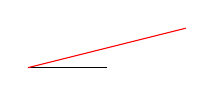
\begin{tikzpicture}
  \draw                            (0,0) -- (1,0);
  \draw[x={(2cm,0.5cm)},color=red] (0,0) -- (1,0);
\end{tikzpicture}
\end{codeexample}

    You can use this, for example, to exchange the meaning of the $x$- and
    $y$-coordinate.
    
    您可以使用此选项,例如,交换 $x$-和 $y$-坐标的含义。

\begin{codeexample}[]
\begin{tikzpicture}[smooth]
  \draw plot coordinates{(1,0) (2,0.5) (3,0) (3,1)};
  \draw[x={(0cm,1cm)},y={(1cm,0cm)},color=red]
        plot coordinates{(1,0) (2,0.5) (3,0) (3,1)};
\end{tikzpicture}
\end{codeexample}
    %
\end{key}

\begin{key}{/tikz/y=\meta{value} (initially 1cm)}
    Works like the |x=| option, only if \meta{value} is a dimension, the
    resulting vector points to $(0,\meta{value})$.

    和 |x=| 选项相同,但如果 \meta{value} 是一个尺寸,则生成的向量指向 $(0,\meta{value})$。

\end{key}

\begin{key}{/tikz/z=\meta{value} (initially \normalfont$-3.85$mm)}
    Works like the |y=| option, but now a dimension is the point
    $(\meta{value},\meta{value})$.
    
    类似于 |y=| 选项,但现在尺寸是点 $(\meta{value},\meta{value})$。

\begin{codeexample}[]
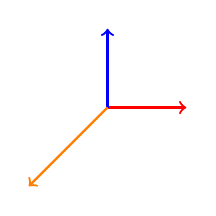
\begin{tikzpicture}[z=-1cm,->,thick]
  \draw[color=red] (0,0,0) -- (1,0,0);
  \draw[color=blue] (0,0,0) -- (0,1,0);
  \draw[color=orange] (0,0,0) -- (0,0,1);
\end{tikzpicture}
\end{codeexample}
    %
\end{key}


\subsection{Coordinate Transformations\\坐标变换}

\pgfname\ and \tikzname\ allow you to specify \emph{coordinate
transformations}. Whenever you specify a coordinate as in |(1,0)| or
|(1cm,1pt)| or |(30:2cm)|, this coordinate is first ``reduced'' to a position
of the form ``$x$ points to the right and $y$ points upwards''. For example,
|(1in,5pt)| is reduced to ``$72\frac{72}{100}$ points to the right and 5 points
upwards'' and |(90:100pt)| means ``0pt to the right and 100 points upwards''.

\pgfname\ 和 \tikzname\ 允许您指定\emph{坐标变换}。每当您指定一个坐标,例如 |(1,0)| 或 |(1cm,1pt)| 或 |(30:2cm)|,此坐标首先被“缩减”为形式“$x$指向右侧,$y$指向上方”的位置。例如,|(1in,5pt)| 被缩减为“向右移动$72\frac{72}{100}$点,向上移动5点”,而 |(90:100pt)| 表示“向右移动0点,向上移动100点”。

The next step is to apply the current \emph{coordinate transformation matrix}
to the coordinate. For example, the coordinate transformation matrix might
currently be set such that it adds a certain constant to the $x$ value. Also,
it might be set up such that it, say, exchanges the $x$ and $y$ value. In
general, any ``standard'' transformation like translation, rotation, slanting,
or scaling or any combination thereof is possible. (Internally, \pgfname\ keeps
track of a coordinate transformation matrix very much like the concatenation
matrix used by \textsc{pdf} or PostScript.)

下一步是将当前的\emph{坐标变换矩阵}应用于坐标。例如,当前的坐标变换矩阵可能被设置为在$x$值上添加某个常数。此外,它也可能被设置为交换$x$值和$y$值。一般来说,任何“标准”的变换,如平移、旋转、倾斜或缩放,或其任意组合都是可能的。(在内部,\pgfname\ 类似于\textsc{pdf}或PostScript使用的连接矩阵跟踪坐标变换矩阵。)


\begin{codeexample}[]
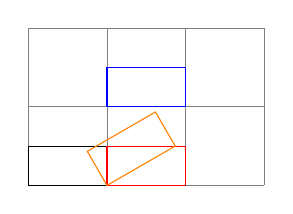
\begin{tikzpicture}
  \draw[help lines] (0,0) grid (3,2);
  \draw (0,0) rectangle (1,0.5);
  \begin{scope}[xshift=1cm]
    \draw             [red]    (0,0) rectangle (1,0.5);
    \draw[yshift=1cm] [blue]   (0,0) rectangle (1,0.5);
    \draw[rotate=30]  [orange] (0,0) rectangle (1,0.5);
  \end{scope}
\end{tikzpicture}
\end{codeexample}

The most important aspect of the coordinate transformation matrix is \emph{that
it applies to coordinates only!} In particular, the coordinate transformation
has no effect on things like the line width or the dash pattern or the shading
angle. In certain cases, it is not immediately clear whether the coordinate
transformation matrix \emph{should} apply to a certain dimension. For example,
should the coordinate transformation matrix apply to grids? (It does.) And what
about the size of arced corners? (It does not.) The general rule is: ``If there
is no `coordinate' involved, even `indirectly', the matrix is not applied.''.
However, sometimes, you simply have to try or look it up in the documentation
whether the matrix will be applied.

坐标变换矩阵最重要的方面是\emph{它仅适用于坐标!}特别地,坐标变换对线宽、虚线模式或渐变角度等没有影响。在某些情况下,不清楚坐标变换矩阵是否\emph{应该}应用于某个维度。例如,坐标变换矩阵是否应该应用于网格?(是的。)那么弧形拐角的尺寸呢?(不应用。)一般规则是:“如果没有涉及‘坐标’,即使是间接的,矩阵也不会应用。”但是,有时您只需要尝试或查阅文档,以确定矩阵是否将被应用。

Setting the matrix cannot be done directly. Rather, all you can do is to
``add'' another transformation to the current matrix. However, all
transformations are local to the current \TeX-group. All transformations are
added using graphic options, which are described below.

不能直接设置矩阵。您只能向当前矩阵“添加”另一个变换。但是,所有变换都局限于当前的\TeX 组。所有变换都使用图形选项添加,下面将对其进行描述。

Transformations apply immediately when they are encountered ``in the middle of
a path'' and they apply only to the coordinates on the path following the
transformation option.

当遇到变换时,它们会立即应用于“路径中间”,并且仅对变换选项后面的路径上的坐标应用。

%
\begin{codeexample}[]
\tikz \draw (0,0) rectangle (1,0.5) [xshift=2cm] (0,0) rectangle (1,0.5);
\end{codeexample}

A final word of warning: You should refrain from using ``aggressive''
transformations like a scaling of a factor of 10\,000. The reason is that all
transformations are done using \TeX, which has a fairly low accuracy.
Furthermore, in certain situations it is necessary that \tikzname\
\emph{inverts} the current transformation matrix and this will fail if the
transformation matrix is badly conditioned or even singular (if you do not know
what singular matrices are, you are blessed).

最后要警告一句:您应该避免使用“激进”的变换,如缩放因子为 10,000。原因是所有的变换都是使用 \TeX 进行的,而 \TeX 的精度相对较低。此外,在某些情况下,\tikzname\ 需要\emph{反转}当前的变换矩阵,如果变换矩阵条件不好或甚至是奇异的(如果您不知道奇异矩阵是什么,那就幸运)。

\begin{key}{/tikz/shift={\ttfamily\char`\{}\meta{coordinate}{\ttfamily\char`\}}}
    Adds the \meta{coordinate} to all coordinates.
    
    添加\meta{coordinate}到所有坐标。


\begin{codeexample}[]
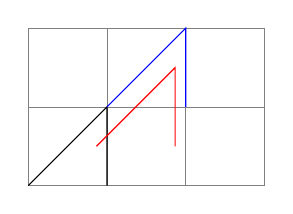
\begin{tikzpicture}
  \draw[help lines] (0,0) grid (3,2);
  \draw                       (0,0) -- (1,1) -- (1,0);
  \draw[shift={(1,1)},blue]   (0,0) -- (1,1) -- (1,0);
  \draw[shift={(30:1cm)},red] (0,0) -- (1,1) -- (1,0);
\end{tikzpicture}
\end{codeexample}
    %
\end{key}

\begin{key}{/tikz/shift only}
    This option does not take any parameter. Its effect is to cancel all
    current transformations except for the shifting. This means that the origin
    will remain where it is, but any rotation around the origin or scaling
    relative to the origin or skewing will no longer have an effect.

    此选项不带任何参数。它的作用是取消除了平移之外的所有当前变换。这意味着原点将保持在原位,但是对原点周围的旋转、缩放或扭曲将不再产生影响。

    This option is useful in situations where a complicated transformation is
    used to ``get to a position'', but you then wish to draw something
    ``normal'' at this position.
    
    在需要使用复杂变换“到达某个位置”,但是您希望在该位置绘制“正常”内容的情况下,此选项非常有用。


\begin{codeexample}[]
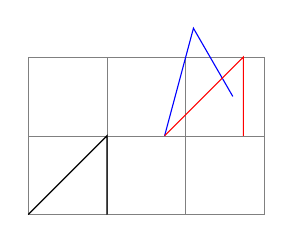
\begin{tikzpicture}
  \draw[help lines] (0,0) grid (3,2);
  \draw                                      (0,0) -- (1,1) -- (1,0);
  \draw[rotate=30,xshift=2cm,blue]           (0,0) -- (1,1) -- (1,0);
  \draw[rotate=30,xshift=2cm,shift only,red] (0,0) -- (1,1) -- (1,0);
\end{tikzpicture}
\end{codeexample}
    %
\end{key}

\begin{key}{/tikz/xshift=\meta{dimension}}
    Adds \meta{dimension} to the $x$ value of all coordinates.
    
    将\meta{dimension}添加到所有坐标的$x$值。


\begin{codeexample}[]
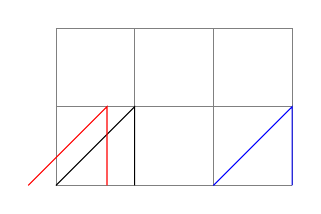
\begin{tikzpicture}
  \draw[help lines] (0,0) grid (3,2);
  \draw                   (0,0) -- (1,1) -- (1,0);
  \draw[xshift=2cm,blue]  (0,0) -- (1,1) -- (1,0);
  \draw[xshift=-10pt,red] (0,0) -- (1,1) -- (1,0);
\end{tikzpicture}
\end{codeexample}
    %
\end{key}

\begin{key}{/tikz/yshift=\meta{dimension}}
    Adds \meta{dimension} to the $y$ value of all coordinates.

    将\meta{dimension}添加到所有坐标的$y$值。

\end{key}

\begin{key}{/tikz/scale=\meta{factor}}
    Multiplies all coordinates by the given \meta{factor}. The \meta{factor}
    should not be excessively large in absolute terms or very close to zero.
    
    将所有坐标乘以给定的\meta{factor}。\meta{factor}的绝对值不应该过大,也不应该非常接近零。

\begin{codeexample}[]
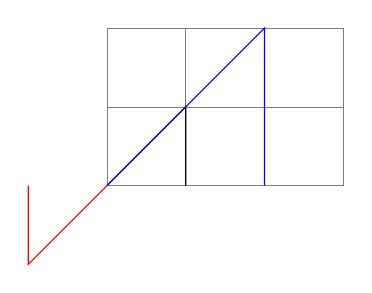
\begin{tikzpicture}
  \draw[help lines] (0,0) grid (3,2);
  \draw               (0,0) -- (1,1) -- (1,0);
  \draw[scale=2,blue] (0,0) -- (1,1) -- (1,0);
  \draw[scale=-1,red] (0,0) -- (1,1) -- (1,0);
\end{tikzpicture}
\end{codeexample}
    %
\end{key}

\begin{key}{/tikz/scale around={\ttfamily\char`\{}\meta{factor}|:|\meta{coordinate}{\ttfamily\char`\}}}
    Scales the coordinate system by \meta{factor}, with the ``origin of
    scaling'' centered on \meta{coordinate} rather than the origin.
    
    以\meta{factor}为比例缩放坐标系,以\meta{coordinate}为中心的“缩放原点”,而不是以原点为中心。
\begin{codeexample}[]
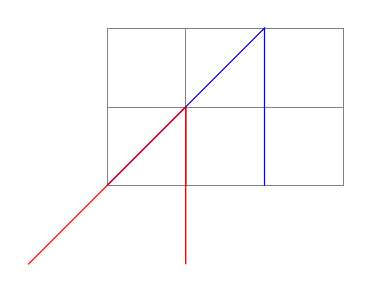
\begin{tikzpicture}
  \draw[help lines] (0,0) grid (3,2);
  \draw                             (0,0) -- (1,1) -- (1,0);
  \draw[scale=2,blue]               (0,0) -- (1,1) -- (1,0);
  \draw[scale around={2:(1,1)},red] (0,0) -- (1,1) -- (1,0);
\end{tikzpicture}
\end{codeexample}
    %
\end{key}

\begin{key}{/tikz/xscale=\meta{factor}}
    Multiplies only the $x$-value of all coordinates by the given
    \meta{factor}.

    仅将所有坐标的$x$值乘以给定的\meta{factor}。

\begin{codeexample}[]
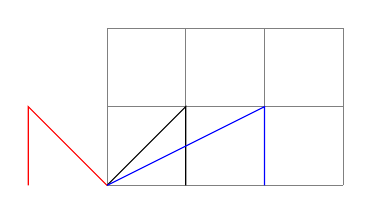
\begin{tikzpicture}
  \draw[help lines] (0,0) grid (3,2);
  \draw                (0,0) -- (1,1) -- (1,0);
  \draw[xscale=2,blue] (0,0) -- (1,1) -- (1,0);
  \draw[xscale=-1,red] (0,0) -- (1,1) -- (1,0);
\end{tikzpicture}
\end{codeexample}
    %
\end{key}

\begin{key}{/tikz/yscale=\meta{factor}}
    Multiplies only the $y$-value of all coordinates by \meta{factor}.

    仅将所有坐标的$y$值乘以\meta{factor}。

\end{key}

\begin{key}{/tikz/xslant=\meta{factor}}
    Slants the coordinate horizontally by the given \meta{factor}:
    
    将坐标水平倾斜给定的\meta{factor}:

\begin{codeexample}[]
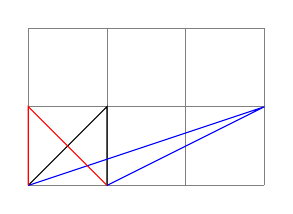
\begin{tikzpicture}
  \draw[help lines] (0,0) grid (3,2);
  \draw                (0,0) -- (1,1) -- (1,0);
  \draw[xslant=2,blue] (0,0) -- (1,1) -- (1,0);
  \draw[xslant=-1,red] (0,0) -- (1,1) -- (1,0);
\end{tikzpicture}
\end{codeexample}
    %
\end{key}

\begin{key}{/tikz/yslant=\meta{factor}}
    Slants the coordinate vertically by the given \meta{factor}:
    
    将坐标垂直倾斜给定的\meta{factor}:

\begin{codeexample}[]
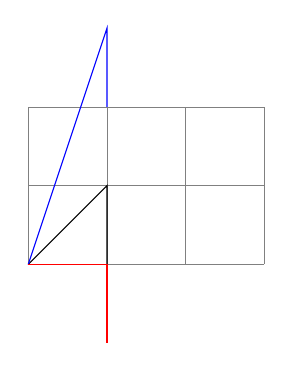
\begin{tikzpicture}
  \draw[help lines] (0,0) grid (3,2);
  \draw                (0,0) -- (1,1) -- (1,0);
  \draw[yslant=2,blue] (0,0) -- (1,1) -- (1,0);
  \draw[yslant=-1,red] (0,0) -- (1,1) -- (1,0);
\end{tikzpicture}
\end{codeexample}
    %
\end{key}

\begin{key}{/tikz/rotate=\meta{degree}}
    Rotates the coordinate system by \meta{degree}:
    
    将坐标系按\meta{degree}旋转:
\begin{codeexample}[]
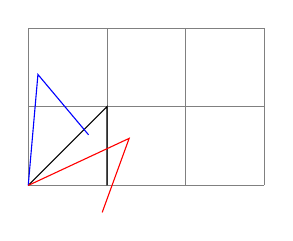
\begin{tikzpicture}
  \draw[help lines] (0,0) grid (3,2);
  \draw                 (0,0) -- (1,1) -- (1,0);
  \draw[rotate=40,blue] (0,0) -- (1,1) -- (1,0);
  \draw[rotate=-20,red] (0,0) -- (1,1) -- (1,0);
\end{tikzpicture}
\end{codeexample}
    %
\end{key}

\begin{key}{/tikz/rotate around={\ttfamily\char`\{}\meta{degree}|:|\meta{coordinate}{\ttfamily\char`\}}}
    Rotates the coordinate system by \meta{degree} around the point
    \meta{coordinate}.
    
    将坐标系围绕\meta{coordinate}点按\meta{degree}旋转。
\begin{codeexample}[]
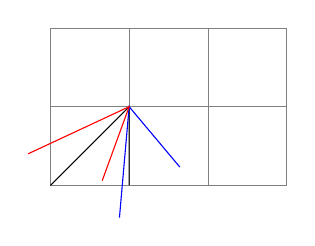
\begin{tikzpicture}
  \draw[help lines] (0,0) grid (3,2);
  \draw                                (0,0) -- (1,1) -- (1,0);
  \draw[rotate around={40:(1,1)},blue] (0,0) -- (1,1) -- (1,0);
  \draw[rotate around={-20:(1,1)},red] (0,0) -- (1,1) -- (1,0);
\end{tikzpicture}
\end{codeexample}
    %
\end{key}

\begin{key}{/tikz/rotate around x=\meta{angle}}
    This key sets the $x$, $y$ and $z$ vectors of the \pgfname\
    $xyz$-coordinate system so that they are rotated by \meta{angle} around the
    axis corresponding to the $x$-vector. The rotation is applied so that when
    looking towards the origin along this axis, positive angles result in an
    anticlockwise rotation.
    
    此键设置\pgfname 的$xyz$坐标系的$x$、$y$和$z$向量,使它们围绕与$x$向量对应的轴旋转\meta{angle}。旋转应用于当沿着此轴朝向原点时,正角度会产生逆时针旋转。
\begin{codeexample}[]
\begin{tikzpicture}[>=stealth]
  \draw [->] (0,0,0) -- (2,0,0) node [at end, right] {$x$};
  \draw [->] (0,0,0) -- (0,2,0) node [at end, left]  {$y$};
  \draw [->] (0,0,0) -- (0,0,2) node [at end, left]  {$z$};

  \draw [red,   rotate around x=0]  (0,0,0) -- (1,1,0) -- (1,0,0);
  \draw [green, rotate around x=45] (0,0,0) -- (1,1,0) -- (1,0,0);
  \draw [blue,  rotate around x=90] (0,0,0) -- (1,1,0) -- (1,0,0);
\end{tikzpicture}
\end{codeexample}
    %
\end{key}

\begin{key}{/tikz/rotate around y=\meta{angle}}
    This key sets the $x$, $y$ and $z$ vectors of the \pgfname\
    $xyz$-coordinate system so that they are rotated by \meta{angle} around
    the axis corresponding to the $y$-vector. The rotation is applied so that
    when looking towards the origin along this axis, positive angles result in
    an anticlockwise rotation.
    
    此键设置\pgfname 的$xyz$坐标系的$x$、$y$和$z$向量,使它们围绕与$y$向量对应的轴旋转\meta{angle}。旋转应用于当沿着此轴朝向原点时,正角度会产生逆时针旋转。
\begin{codeexample}[]
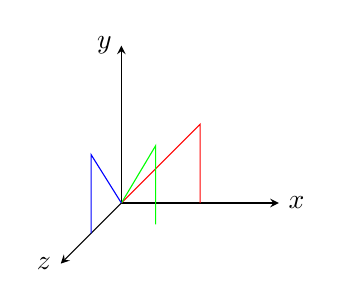
\begin{tikzpicture}[>=stealth]
  \draw [->] (0,0,0) -- (2,0,0) node [at end, right] {$x$};
  \draw [->] (0,0,0) -- (0,2,0) node [at end, left]  {$y$};
  \draw [->] (0,0,0) -- (0,0,2) node [at end, left]  {$z$};

  \draw [red,   rotate around y=0]   (0,0,0) -- (1,1,0) -- (1,0,0);
  \draw [green, rotate around y=-45] (0,0,0) -- (1,1,0) -- (1,0,0);
  \draw [blue,  rotate around y=-90] (0,0,0) -- (1,1,0) -- (1,0,0);
\end{tikzpicture}
\end{codeexample}
    %
\end{key}

\begin{key}{/tikz/rotate around z=\meta{angle}}
    This key sets the $x$, $y$ and $z$ vectors of the \pgfname\
    $xyz$-coordinate system so that they are rotated by \meta{angle} around the
    axis corresponding to the $z$-vector. The rotation is applied so that when
    looking towards the origin along this axis, positive angles result in an
    anticlockwise rotation.
    
    此键设置\pgfname 的$xyz$坐标系的$x$、$y$和$z$向量,使它们围绕与$z$向量对应的轴旋转\meta{angle}。旋转应用于当沿着此轴朝向原点时,正角度会产生逆时针旋转。

\begin{codeexample}[]
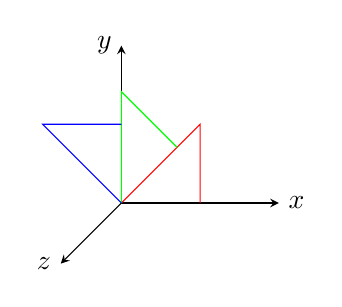
\begin{tikzpicture}[>=stealth]
  \draw [->] (0,0,0) -- (2,0,0) node [at end, right] {$x$};
  \draw [->] (0,0,0) -- (0,2,0) node [at end, left]  {$y$};
  \draw [->] (0,0,0) -- (0,0,2) node [at end, left]  {$z$};

  \draw [red,   rotate around z=0]  (0,0) -- (1,1) -- (1,0);
  \draw [green, rotate around z=45] (0,0) -- (1,1) -- (1,0);
  \draw [blue,  rotate around z=90] (0,0) -- (1,1) -- (1,0);
\end{tikzpicture}
\end{codeexample}
    %
\end{key}

\begin{key}{/tikz/cm={\ttfamily\char`\{}\meta{$a$}|,|\meta{$b$}|,|\meta{$c$}|,|\meta{$d$}|,|\meta{coordinate}{\ttfamily\char`\}}}
    applies the following transformation to all coordinates: Let $(x,y)$ be the
    coordinate to be transformed and let \meta{coordinate} specify the point
    $(t_x,t_y)$. Then the new coordinate is given by
    $\left(\begin{smallmatrix} a & c \\ b & d\end{smallmatrix}\right)
    \left(\begin{smallmatrix} x \\ y \end{smallmatrix}\right) +
    \left(\begin{smallmatrix} t_x \\ t_y \end{smallmatrix}\right)$.
    Usually, you do not use this option directly.
    %

    对所有坐标应用以下变换:设$(x,y)$为要进行变换的坐标,\meta{coordinate}指定点$(t_x,t_y)$。则新坐标由$\left(\begin{smallmatrix} a & c \\ b & d\end{smallmatrix}\right)\left(\begin{smallmatrix} x \\ y \end{smallmatrix}\right)+\left(\begin{smallmatrix} t_x \\ t_y \end{smallmatrix}\right)$给出。通常,您不直接使用此选项。

\begin{codeexample}[]
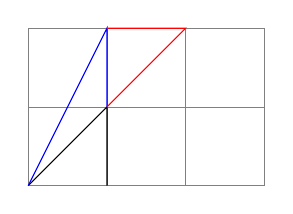
\begin{tikzpicture}
  \draw[help lines] (0,0) grid (3,2);
  \draw                             (0,0) -- (1,1) -- (1,0);
  \draw[cm={1,1,0,1,(0,0)},blue]    (0,0) -- (1,1) -- (1,0);
  \draw[cm={0,1,1,0,(1cm,1cm)},red] (0,0) -- (1,1) -- (1,0);
\end{tikzpicture}
\end{codeexample}
    %
\end{key}

\begin{key}{/tikz/reset cm}
    Completely resets the coordinate transformation matrix to the identity
    matrix. This will destroy not only the transformations applied in the
    current scope, but also all transformations inherited from surrounding
    scopes. Do not use this option, unless you really, really know what you are
    doing.

    完全重置坐标变换矩阵为单位矩阵。这将不仅销毁当前作用域中应用的变换,还会销毁从周围作用域继承的所有变换。除非您确实非常了解自己在做什么,否则不要使用此选项。


\end{key}


\subsection{Canvas Transformations\\画布变换}

A \emph{canvas transformation}, see
Section~\ref{section-design-transformations} for details, is best thought of as
a transformation in which the drawing canvas is stretched or rotated. Imaging
writing something on a balloon (the canvas) and then blowing air into the
balloon: Not only does the text become larger, the thin lines also become
larger. In particular, if you scale the canvas by a factor of two, all lines
are twice as thick.

画布变换,见第~\ref{section-design-transformations} 节了解详情,最好将其视为画布被拉伸或旋转的变换。想象一下,在气球上写字(画布),然后将空气吹入气球中:不仅文字变大,细线也变粗。特别地,如果将画布缩放两倍,所有线条的粗细都会增加一倍。

Canvas transformations should be used with great care. In most circumstances
you do \emph{not} want line widths to change in a picture as this creates
visual inconsistency.

画布变换应谨慎使用。在大多数情况下,您\emph{不希望}图片中的线宽发生变化,因为这会导致视觉上的不一致。

Just as important, when you use canvas transformations \emph{\pgfname\ loses
track of positions of nodes and of picture sizes} since it does not take the
effect of canvas transformations into account when it computes coordinates of
nodes (do not, however, rely on this; it may change in the future).

同样重要的是,当您使用画布变换时,\emph{\pgfname\ 会丢失节点的位置和图片的大小},因为在计算节点的坐标时,它不考虑画布变换的效果(不过,请不要依赖这一点;它可能在将来发生变化)。

Finally, note that a canvas transformation always applies to a path as a whole,
it is not possible (as for coordinate transformations) to use different
transformations in different parts of a path.

最后,请注意,画布变换始终应用于整个路径,不可能(就像坐标变换一样)在路径的不同部分使用不同的变换。

In short, you should not use canvas transformations unless you really know what
you are doing.

简而言之,除非您确实了解自己在做什么,否则不应使用画布变换。

\begin{key}{/tikz/transform canvas=\meta{options}}
    The \meta{options} should contain coordinate transformations options like
    |scale| or |xshift|. Multiple options can be given, their effects
    accumulate in the usual manner. The effect of these \meta{options}
    (immediately) changes the current canvas transformation matrix. The
    coordinate transformation matrix is not changed. Tracking of the picture
    size is (locally) switched off and the node coordinate will no longer be
    correct.
    
    \meta{options} 应包含坐标变换选项,如 |scale| 或 |xshift|。可以给出多个选项,它们的效果按照通常的方式累积。这些 \meta{options} 的效果(立即)改变了当前的画布变换矩阵。坐标变换矩阵不会改变。图片大小的跟踪被(局部地)关闭,并且节点坐标将不再正确。
\begin{codeexample}[]
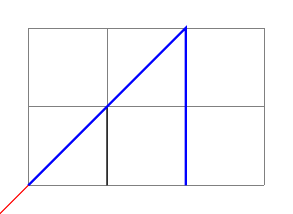
\begin{tikzpicture}
  \draw[help lines] (0,0) grid (3,2);
  \draw                                    (0,0) -- (1,1) -- (1,0);
  \draw[transform canvas={scale=2},blue]   (0,0) -- (1,1) -- (1,0);
  \draw[transform canvas={rotate=180},red] (0,0) -- (1,1) -- (1,0);
\end{tikzpicture}
\end{codeexample}
    %
\end{key}
